\documentclass[12pt,a4paper]{report}

% --- Paquetes de Idioma y Codificación ---
\usepackage[utf8]{inputenc}
\usepackage[T1]{fontenc}
\usepackage[spanish, es-tabla]{babel}

% --- Diseño de Página ---
\usepackage{geometry}
\geometry{top=2.5cm, bottom=2.5cm, left=3cm, right=3cm}

% --- Matemáticas y Símbolos ---
\usepackage{amsmath, amssymb, amsthm}

% --- Colores y Cajas ---
\usepackage[dvipsnames]{xcolor}
\usepackage[most]{tcolorbox}

% Caption

\usepackage{caption}

% Gráficos

\usepackage{graphicx}

% Espaciadora

\newcommand{\esp}{\vspace{0.5cm}}

% promedio

\newcommand{\prom}[1]{\left\langle #1 \right\rangle}

% ket

\newcommand{\ket}[1]{| #1 \rangle}

% bra

\newcommand{\bra}[1]{\langle #1 |}

% braket

\newcommand{\braket}[2]{\langle #1 | #2 \rangle}

% Bibliografía

\usepackage[style=apa, backend=biber]{biblatex} % Estilo APA
\addbibresource{biblio.bib} % Nombre de tu archivo .bib

% Configuración de cajas personalizadas
\newtcolorbox{importante}{
	colback=red!5!white,
	colframe=red!75!black,
	title=Importante,
	fonttitle=\bfseries
}

\newtcolorbox{nota}{
	colback=blue!5!white,
	colframe=blue!75!black,
	title=Nota,
	fonttitle=\bfseries
}

% Definición de la caja de bibliografía
\newtcolorbox{bibliografia}{
	colback=gray!5!white,
	colframe=gray!75!black,
	title=Bibliografías útiles,
	fonttitle=\bfseries,
	breakable
}

% Socrative para óptica 2

\newtcolorbox{Socrative}{
	colback=orange!5!white,
	colframe=orange!75!black,
	title=Socrative,
	fonttitle=\bfseries,
	breakable
}

% Float

\usepackage{float}

% --- Hipervínculos ---
\usepackage{hyperref}
\hypersetup{
	colorlinks=true,
	linkcolor=blue,
	filecolor=magenta,      
	urlcolor=cyan,
}

% --- Datos del Documento ---
\title{Stadistical Physics }
\author{Chengyu Jin}
\date{\today}

\begin{document}
	
	\maketitle
	
	\tableofcontents
	\newpage
	
	\chapter{Classical atomic gas}
	
	\section{Ideal systems}
	
	\noindent In an ideal system I can express the system's hamiltonian as
	
	\esp
	
	\begin{equation}
		H = \sum_i h_i
	\end{equation}
	
	\esp
	
	\noindent Applying this in the canonical ensemble framework's probability we have
	
	\esp
	
	\begin{equation}
		p(C) = \frac{e^{\beta H(C)}}{Z} = \frac{e^{\beta \sum_i h_i}}{Z} = \prod _i \frac{e^{\beta h_i}}{Z}
	\end{equation}
	
	\esp
	
	\begin{nota}
		The previous result is consistence with the stadistical result: if $A \cap B = {0}$ then $P(A\cup B)=P(A)P(B)$
	\end{nota}
	
	\subsection{Examples}
	
	If we have a potential $V(r_{ij})$, this is a potential that depends on the relative position of the particle i with particles j. I cannot separate the hamiltonian because the particle i dependes on surrounding particles.
	
	\esp
	
	\begin{equation}
		V(r_{ij}) \implies H \neq \sum_i h_i
	\end{equation}
	
	\esp
	
	If we have a potential $V(r_i)$, this is a potential that only depends on the particle's position. Then I can separate the hamiltonian.
	
	\esp
	
	\begin{equation}
		V(r_i) \implies H = \sum_i h_i = \sum_i \frac{p_i^2}{2m_i} + \sum_i V(r_i)
	\end{equation}
	
	\esp
	
	The Ising Model that we have seen in Computational Physics has the following hamiltonian
	
	\esp
	
	\begin{equation}
		H = -\frac{J}{2} \sum_{ij}^N s_{ij} (s_{i+1,j}+s_{i-1,j}+s_{i,j+1}+s_{i,j-1})
	\end{equation}
	
	\esp
	
	As we can see in the equation, the hamiltonian of the particle i-j depend on the surrounding, then we cannot express the hamiltonian as sums of each particles' hamiltonians.
	
	\esp
	
	\begin{equation}
		H = -\frac{J}{2} \sum_{ij}^N s_{ij} (s_{i+1,j}+s_{i-1,j}+s_{i,j+1}+s_{i,j-1}) \neq \sum_i h_i
	\end{equation}
	
	\esp
	
	If we have the following hamiltonian, we can separate it in sum of particles' hamiltonian with $h_i=-Js_i$.
	
	\esp
	
	\begin{equation}
		H = -J \sum_i s_i = \sum_i h_i = \sum_i -Js_i
	\end{equation}
	
	\esp
	
	\section{Boltzmann Gas}
	
	\noindent The Boltzmann Gas it is the common limit of fermions and bosons.
	
	\subsection{In canonical ensemble}
	
	\begin{figure}[H]
		\centering
		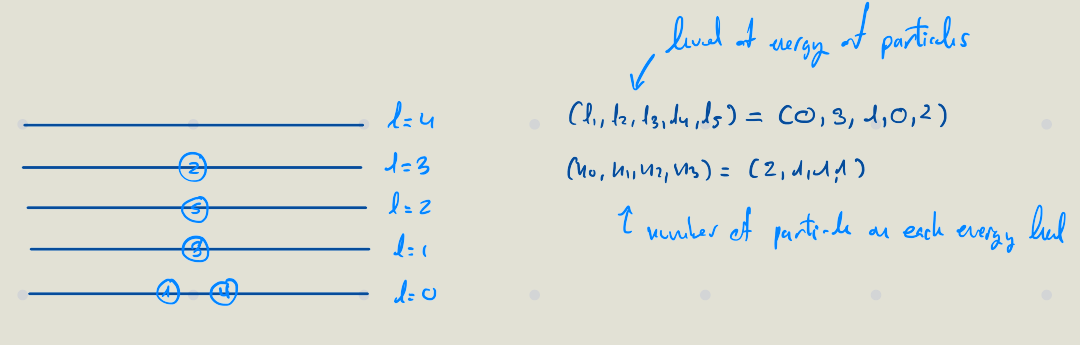
\includegraphics[width=0.7\textwidth]{IMG/bgas.png}
	\end{figure}
	
	\esp
	
	\begin{equation}
		Z = \sum_{\{ n_i \}, \sum_i n_i = N} e^{-\beta E} = \sum_{\{ n_i \}, \sum_i n_i = N} e^{-\beta \sum_i n_i \epsilon_i}
	\end{equation}
	
	\esp
	
	Due to the condition $\sum_i n_i = N$, we cannot calculate the partition function as the sum of partition functions. But we can express the total energy as sum of energy associated to level $l$.
	
	\esp
	
	\begin{equation}
		E = \sum_i n_i \epsilon_i = \sum_i E_{l_i}
	\end{equation}

	\esp
	
	\noindent Applying this in the partition function we obtain
	
	\esp
	
	\begin{equation}
		Z = \sum_{l_1, \dots, l_N} e^{\beta \sum_i \epsilon_{l_i}}
	\end{equation}

	\esp
	
	We need take account the degeneracy. As the particle are \textbf{indistiguishable}, we can consider all the particle as the same, then we only nned to know how to distribuite N same particles in $l$ levels.
	
	\esp
	
	\noindent A set of $\{n_l\}$ correspond $\frac{N!}{\prod_i n_l!}$ possible values of $\{l_1, \dots, l_N\}$.
	
	\esp
	
	\begin{equation}
		Z = \sum_{\{ n_i \}, \sum_i n_i = N} e^{-\beta E} = \sum_{\{ n_i \}, \sum_i n_i = N} \frac{\prod_i n_l!}{N!} e^{-\beta \sum_i n_i \epsilon_i}
	\end{equation}
	
	\esp
	
	\subsection{Boltzmann approximation}
	
	The Boltzmann approximation is $n_l! \approx 1$. This is when $\rho \Lambda_T^3 \ll 1$ with $\Lambda_T^3 = h/\sqrt{2\pi mKT}$. This approximation is good when $T\upuparrows$ or/and $\rho \downdownarrows$ (very diluete cases). Under this condition, bosons and fermions \textbf{behave the same way}.
	
	\esp
	
	\noindent With the Boltzmann approximation, the partition function is
	
	\esp
	
	\begin{equation}
		Z = \sum_i \frac{1}{N!} e^{-\beta \sum_i \epsilon_{l_i}} = \frac{Z_1^N}{N!}
	\end{equation}
	
	\subsection{Particles in a 3D potential well}
	
	\noindent Let's calculate the partition function in this system. Let's assume that
	
	\esp
	
	\begin{equation}
		Z = \sum \frac{1}{N!}(Z_1)^N
	\end{equation}
	
	\esp
	
	\noindent Then let's calculate $Z_1$
	
	\esp
	
	A single particle's energy has two contribution, one due to the traslational degrees of freedom and one due to the internal degrees of freedom.
	
	\esp
	
	\begin{equation}
		\epsilon = \epsilon_{tr} + \epsilon_{in}
	\end{equation}
	
	\esp
	
	\noindent Then the particle function of a single particle is
	
	\esp
	
	\begin{equation}
		Z_1 = \sum_{l_{tr}}\sum_{l_{in}} e^{-\beta \epsilon_{tr}-\beta \epsilon_{in}} = Z_1^{tr} Z_1^{in}
	\end{equation}
	
	\esp
	
	In RAW we developed the solution of Schrödinger's Equation in a potential well in 1D. From this solution we obtained the expression for energy, which is related to the momentum.
	
	\esp
	
	\begin{equation}
		\epsilon = \frac{nh}{4Lm}
	\end{equation}
	
	\esp
	
	\noindent Using this for the traslational energy expression
	
	\esp
	
	\begin{equation}
		\epsilon_{tr} = \frac{p_x^2+p_y^2+p_z^2}{2m} = \frac{\Lambda}{2m}\left(\frac{n_x^2h^2}{4L^2}+\frac{n_y^2h^2}{4L^2}+\frac{n_z^2h^2}{4L^2}\right)
	\end{equation}
	
	\esp
	
	\noindent Let's calculate the partition function
	
	\esp
	
	\begin{equation}
		Z_1^{tr} = \sum_{n_x=1}^{\infty} \sum_{n_y=1}^{\infty} \sum_{n_z=1}^{\infty} e^{-\beta \frac{ h^2}{8mL^2} (n_x^2 + n_y^2 + n_z^2)}
	\end{equation}
	
	\esp
	
	\noindent Let's take a look how to solve individualy
	
	\esp
	
	\begin{equation}
		\sum_{n=1}^{\infty} e^{-\beta \frac{ h^2}{8mL^2}n^2}
	\end{equation}
	
	\esp
	
	If we notice, $p$ is related to the length of the well: $p=hn/2L$, then $\Delta p = p_{n+1}-p_n =h/2L$. If we consider a very large $L$, this is $L\rightarrow\infty$ then $\Delta p = dp$, let's use this to simplify the summatory. Let's change of variable: $n=pL/h\pi$
	
	\esp
	
	\begin{equation}
		\sum_{n=1}^{\infty} e^{-\beta \frac{ h^2}{8mL^2}n^2} = \sum_{p=\frac{h}{2L}}^{\infty} e^{-\beta \frac{p^2}{2m}}
	\end{equation}
	
	\esp
	
	\noindent We introduce $\Delta p$ in the summatory and we are going to perform a limit, then we can covert the summatory into an integral.
	
	\esp
	
	\begin{equation}
		\underset{\rightarrow \infty}{lim} \sum_{p=\frac{h}{2L}}^{\infty} \frac{2L}{h} \Delta p\ e^{-\beta \frac{p^2}{2m}} = \int_0^{\infty} e^{-\beta \frac{p^2}{2m}}\ dp = \frac{1}{2} \int_{-\infty}^{\infty} e^{-\beta \frac{p^2}{2m}}\ dp
	\end{equation}
	
	\esp
	
	\noindent Substituing the partition function with this integral we have
	
	\esp
	
	\begin{equation}
		\frac{1}{h^3} \int_{-\infty}^{\infty} \int_{-\infty}^{\infty} \int_{-\infty}^{\infty} dp_x \, dp_y \, dp_z \, e^{-\frac{\beta}{2m}(p_x^2 + p_y^2 + p_z^2)}
	\end{equation}
	
	\esp
	
	\noindent Taking into account the Gaussian integral:
	\begin{equation}
		\int_{-\infty}^{\infty} e^{-\frac{x^2}{2\sigma^2}} dx = \sqrt{2\pi\sigma^2}
	\end{equation}
	
	\esp
	
	\noindent It follows that:
	\begin{equation}
		Z_1^{(tr)} = \frac{L^3}{h^3} (2\pi mkT)^{3/2} = \frac{V}{\Lambda_T^3}
	\end{equation}
	
	\esp
	
	\noindent Then the partition funcion is
	
	\esp
	
	\begin{equation}
		Z = \frac{1}{N!}\left(\frac{V}{\Lambda_T^3}\right)^N
	\end{equation}
	
	\esp
	
	\noindent \textbf{The previous result coincide with the classical ideal monoatomic gas.}
	
	\printbibliography[title={Bibliografía}]
\end{document}